%%%%%%%%%%%%%%%%%%%%%%%%%%%%%%%%%%%%%%%%%%%%%%%%%%%%%%%%%%%%%%%%%%%%%%%%%%%%%%%%
%2345678901234567890123456789012345678901234567890123456789012345678901234567890
%        1         2         3         4         5         6         7         8

\documentclass[letterpaper, 10 pt, conference]{ieeeconf}  % Comment this line out if you need a4paper

%\documentclass[a4paper, 10pt, conference]{ieeeconf}      % Use this line for a4 paper

\IEEEoverridecommandlockouts                              % This command is only needed if 
                                                          % you want to use the \thanks command

\overrideIEEEmargins                                      % Needed to meet printer requirements.

\usepackage{graphicx}
\graphicspath{ {/home/robotvision/duckietown/catkin_ws/src/spring2017_nctu/porsche/0560024
} } % Path of image

% See the \addtolength command later in the file to balance the column lengths
% on the last page of the document

% The following packages can be found on http:\\www.ctan.org
%\usepackage{graphics} % for pdf, bitmapped graphics files
%\usepackage{epsfig} % for postscript graphics files
%\usepackage{mathptmx} % assumes new font selection scheme installed
%\usepackage{times} % assumes new font selection scheme installed
%\usepackage{amsmath} % assumes amsmath package installed
%\usepackage{amssymb}  % assumes amsmath package installed

\title{\LARGE \bf
Robotic Vision Project - Object Recognition 
}


\author{Yu-Hsien Chang$^{1}$ and Yu-Ting Lai$^{1}$% <-this % stops a space
\thanks{*This work was not supported by any organization}% <-this % stops a space
\thanks{$^{1}$Yu-Hsien Chang and Yu-Ting Lai are first grade master students in Institute of Electrical and Control Engineering, National Chiao Tung University, HsinChu, Taiwan
       }%
}


\begin{document}



\maketitle
\thispagestyle{empty}
\pagestyle{empty}


%%%%%%%%%%%%%%%%%%%%%%%%%%%%%%%%%%%%%%%%%%%%%%%%%%%%%%%%%%%%%%%%%%%%%%%%%%%%%%%%
\begin{abstract}

In this project, we will implement Multi-view Self-supervised Deep Learning for 6D Pose Estimation Algorithm, developed by MIT-Princeton for Amazon Picking Challenge 2016, to recognize objects in images. The Fully Convolutiion Networks used in this algorithm is trained by VGG16 dataset and built with Marvin toolkit. The algoritm can perform object segmentation and pose estimation.

\end{abstract}


%%%%%%%%%%%%%%%%%%%%%%%%%%%%%%%%%%%%%%%%%%%%%%%%%%%%%%%%%%%%%%%%%%%%%%%%%%%%%%%%
\section{INTRODUCTION}

~\cite{7354005}
~\cite{7353560}
~\cite{7758087}
~\cite{6907778}
~\cite{7354243}

Robotic Grasping is a cruical task in the real world, it is composed of object recognition and pose estimation in order to grasp objects successfully.Object Recognition is and aplication to recognize objects in the view and it has two phases, one is ofline learning phase and the other is online recognizing phase. It can improve the efficiency in warehouse and reduce labor force. This technique is not only interesting but also useful in many scenarios. However, its performance will encounter difficulties due to different view points, various light conditions and transparent objects. We implement Multi-view Self-supervised Deep Learning for 6D Pose Estimation in the project and solve the difficulties mentioned above.
Therefore, we first captured images using Intel RealSense SR300, then do the image segmentation to find the location of known objects using Fully Convolution Network(FCN). After getting the confidence score from the FCN, the pose estimation algorithm predict the pose of the objects. Bounding boxes are drawn on the RGB images for visualizing the result. 
The organization of the report is as follows: first, in Section II, we give an overview of Multi-view Self-supervised Deep Learning for 6D Pose Estimation Algorithm. In Section III, we will give a detail explanation of the hardware and the algorithm we use. Our results will be shown in Section IV. Finally, in Section V, we make a conclusion of our work.


\section{RELATED WORK}

\subsection{Amazon Picking Challenge}

It is the competition organized by Amazon Robotics. The goal of the challenge is to strengthen the ties between the industrial and academic robotic communities and promote shared and open solution to some of the big problems in unstructured automation.Each team builds up the hardware on its own and developes the object recognition algorithm and pose estimation algorithm to complete the tasks in the challenge. 

\subsection{Team Delft}

Team Delft was one of 16 finalists for the Amazon Picking Challenge, and it is the championship of APC 2016. Team Delft used two industrial stereo camera's with RGB overlay camera's. One for detection of objects in the tote and the other on the robot gripper to scan the bins. For object recognition, Team Delft used deep learning neural network based on Faster RCNN then performed localization using the implemetation of super4PCS to do global optimation of the pose estimation. Finally, ICP was used to refined the estimation.

\section{TECHNICAL PARTS}

The system architecture is shown in Figure \ref{fig:system_architecture}. We capture RGB images and depth images using Realsense SR300 and Realsense-standalone function provided by MIT-Princeton. Realsense-standalone outputs four information, which are RGB image, raw depth image, image of depth aligned to color and the Cam-Info.txt respectively. RGB images, depth-aligned-to-color images and Cam-Info.txt are used for object recognition and pose estimation. Cam-Info.txt contains camera parameters, such as color intrinsics, depth intrinsics and depth-to-color extrinsics. First, we get HHA features from depth images, in which we address its horizontal disparity, height above ground, and angle between surface normal and gravity to form HHA features. Next, we do image segmentation using pre-trained fully convolutional neural network. In this step, object will be recognized and segmented from the image. After segmentation, we do pose estimation and show the bounding boxes on the RGB images.

\begin{figure}[h]
    \centering
    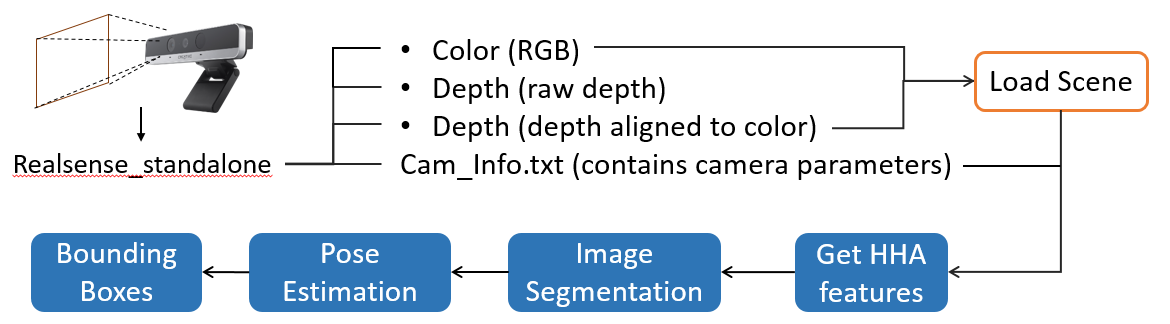
\includegraphics[width=\linewidth]{system_architecture.PNG}
    \caption{System Architecture}
    \label{fig:system_architecture}
\end{figure}

\subsection{Intel Realsense SR300} Intel Realsense SR300, shown in Figure \ref{fig:realsense_sr300}, is a RGB-D camera. In this project, the RGB-D camera is used to capture RGB image and depth image of the target object. Both of the two kinds of image data are used in object segmentation stage and pose estimation stage of the algorithm. The resolution of RGB image is 640*480 pixels and the resolution of depth image is 640*480 pixels. The range of depth capturing is 0.2m to 1.5m. 

\begin{figure}[h]
    \centering
    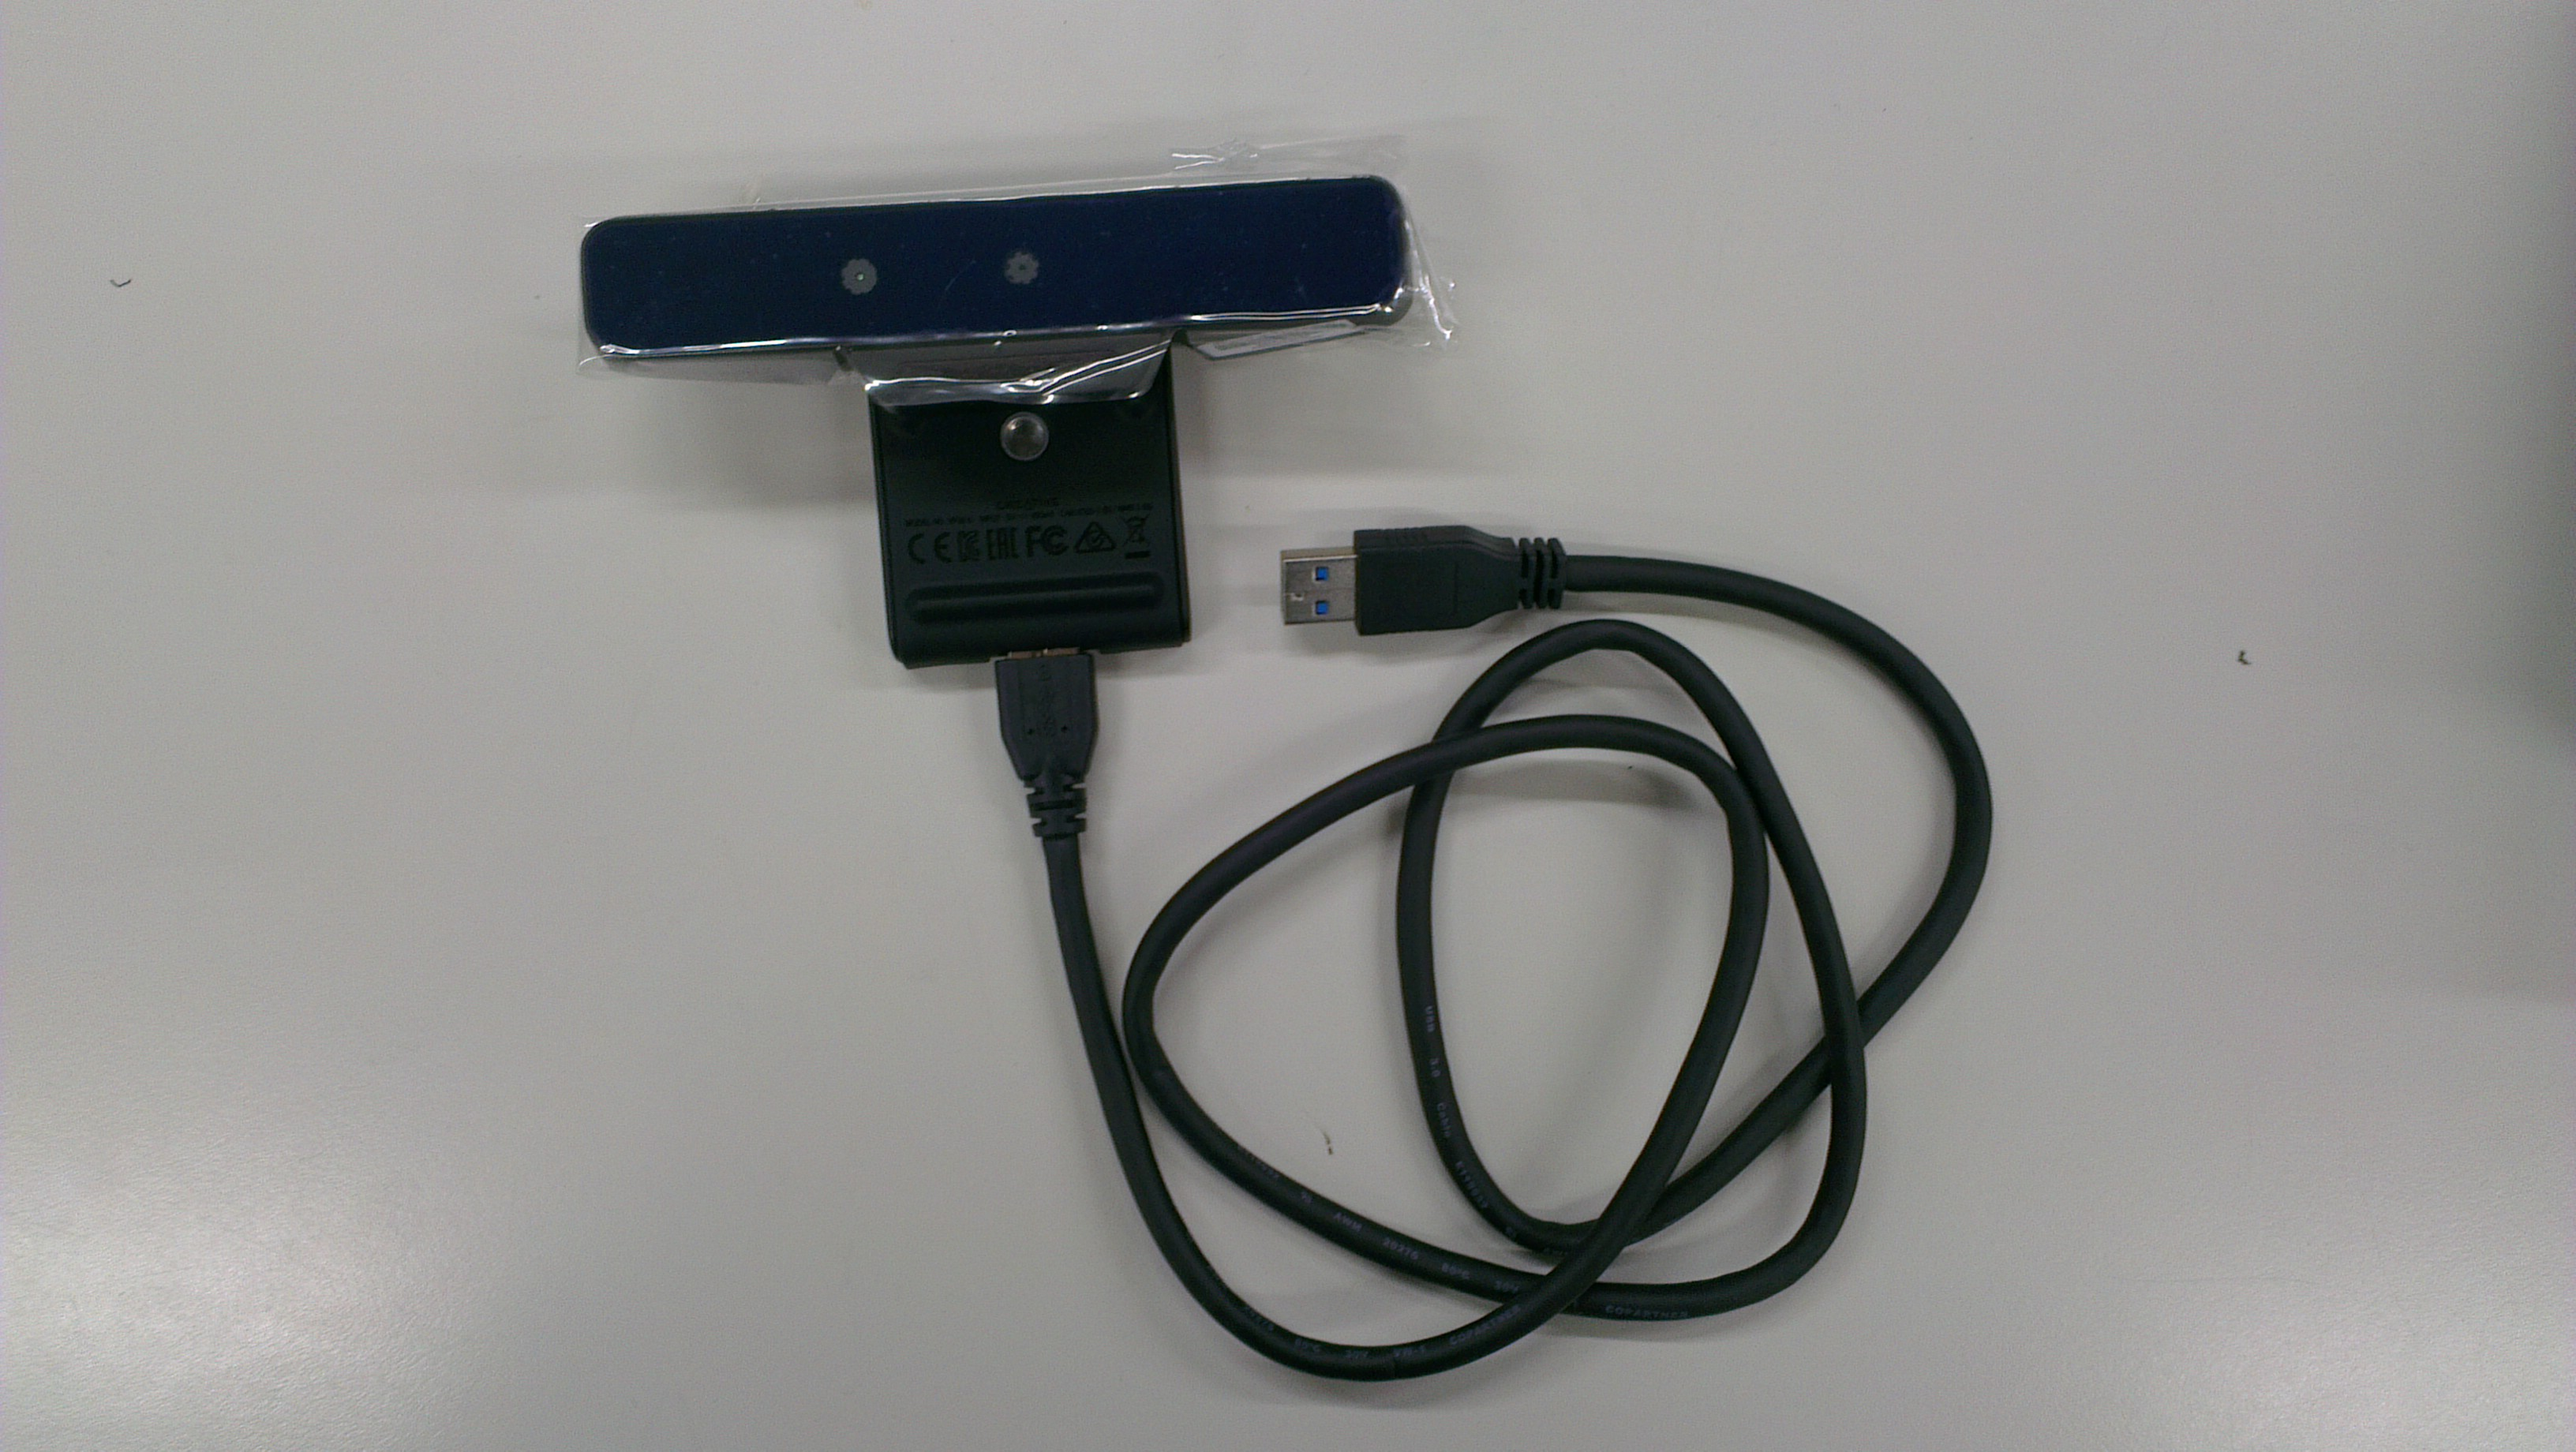
\includegraphics[width=\linewidth]{realsense_sr300.JPEG}
    \caption{Intel Realsense SR300}
    \label{fig:realsense_sr300}
\end{figure}


\subsection{Object Segmentation}

After we captured depth images from realsense, we extract the HHA features from them. HHA features are self-defined features, which address horizontal disparity, height above ground, and angle between surface normal and gravity, for each point. We will create a HHA map like figure \ref{fig:HHA}. The higher intensity means the point has a greater value of the sum of these three features. Then, we see this HHA feature map as the input to the pre-trained neural network. The neural network was trained using Marvin toolkit provided by Princeton. It will output the confidence score of the object with a 16-bit grayscale image. The lighter part in the image indicates that the object is more possible to appear here. Therefore, we complete object segmentation according to every items. For example, if the image contains three objects, it will create three confidence maps. These maps will be used in pose estimation.

\begin{figure}[h]
    \centering
    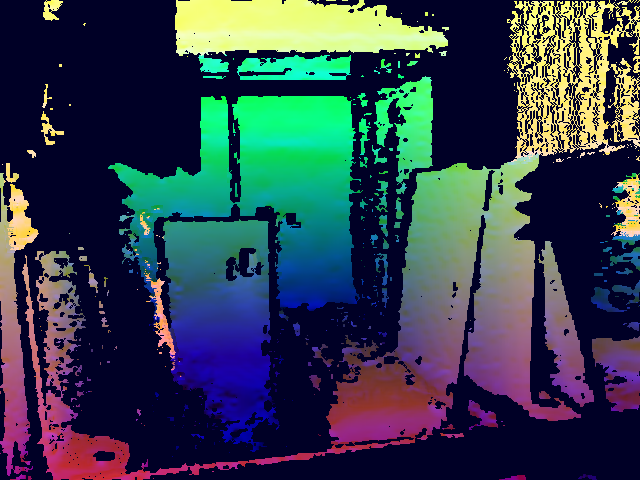
\includegraphics[width=\linewidth]{HHA.PNG}
    \caption{HHA features map}
    \label{fig:HHA}
\end{figure}

\subsection{Pose Estimation} (not yet)

The equations are an exception to the prescribed specifications of this template. You will need to determine whether or not your equation should be typed using either the Times New Roman or the Symbol font (please no other font). To create multileveled equations, it may be necessary to treat the equation as a graphic and insert it into the text after your paper is styled. Number equations consecutively. Equation numbers, within parentheses, are to position flush right, as in (1), using a right tab stop. To make your equations more compact, you may use the solidus ( / ), the exp function, or appropriate exponents. Italicize Roman symbols for quantities and variables, but not Greek symbols. Use a long dash rather than a hyphen for a minus sign. Punctuate equations with commas or periods when they are part of a sentence, as in

$$
\alpha + \beta = \chi \eqno{(1)}
$$

Note that the equation is centered using a center tab stop. Be sure that the symbols in your equation have been defined before or immediately following the equation. Use �(1)�, not �Eq. (1)� or �equation (1)�, except at the beginning of a sentence: �Equation (1) is . . .�

\section{EXPERIMENT}

In this section, we will explain the experiments we did in this project. First, we run the images captured by MIT-Princeton in APC. Second, we will generate the images by ourselves.

\subsection{Benchmark images from APC}

We run the images provided by MIT-Princeton to test the validity of the algorithms. We picked one of the benchmark image set from the shelf in APC scenes. We obtain the HHA features and calculate the confidence map using object segmentation algorithm described above. Next, we predict the poses of the segmented objects by drawing bounding boxes. The results are shown in figure \ref{fig:benchmark_result}.

\begin{figure}[h]
    \centering
    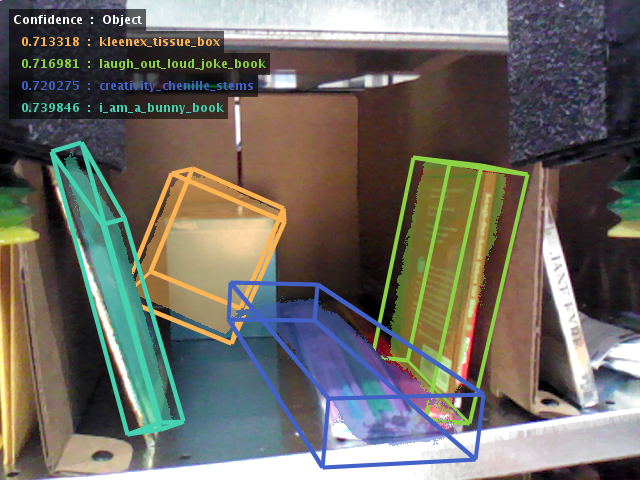
\includegraphics[width=\linewidth]{benchmark_result.png}
    \caption{The results using benchmark images}
    \label{fig:benchmark_result}
\end{figure}

 

\subsection{Self-generated Images} (not yet)

Positioning Figures and Tables: Place figures and tables at the top and bottom of columns. Avoid placing them in the middle of columns. Large figures and tables may span across both columns. Figure captions should be below the figures; table heads should appear above the tables. Insert figures and tables after they are cited in the text. Use the abbreviation �Fig. 1�, even at the beginning of a sentence.

\begin{table}[h]
\caption{An Example of a Table}
\label{table_example}
\begin{center}
\begin{tabular}{|c||c|}
\hline
One & Two\\
\hline
Three & Four\\
\hline
\end{tabular}
\end{center}
\end{table}


   \begin{figure}[thpb]
      \centering
      \framebox{\parbox{3in}{We suggest that you use a text box to insert a graphic (which is ideally a 300 dpi TIFF or EPS file, with all fonts embedded) because, in an document, this method is somewhat more stable than directly inserting a picture.
}}
      %\includegraphics[scale=1.0]{figurefile}
      \caption{Inductance of oscillation winding on amorphous
       magnetic core versus DC bias magnetic field}
      \label{figurelabel}
   \end{figure}
   

Figure Labels: Use 8 point Times New Roman for Figure labels. Use words rather than symbols or abbreviations when writing Figure axis labels to avoid confusing the reader. As an example, write the quantity �Magnetization�, or �Magnetization, M�, not just �M�. If including units in the label, present them within parentheses. Do not label axes only with units. In the example, write �Magnetization (A/m)� or �Magnetization {A[m(1)]}�, not just �A/m�. Do not label axes with a ratio of quantities and units. For example, write �Temperature (K)�, not �Temperature/K.�

\section{CONCLUSIONS}

In this project, we explore the object segmentation and pose estimation algorithms provided MIT-Princeton in Amazon Picking Challenge. We started the whole experiments from setting up Realsense camera to capture depth images, then applying the fully convolutional neural network provided by Marvin toolkit, to pose estimation for the objects. We also captured the images on our own to test the algorithms. However, we need to calculate the exact camera extrinsic parameters between each poses, and calibrate our camera poses with the camera poses in MIT-Princeton. The bounding boxes results are not as good as expected. In the future, we can estimate the exact poses of the objects with a correct calibration parameters. 

\addtolength{\textheight}{-12cm}   % This command serves to balance the column lengths
                                  % on the last page of the document manually. It shortens
                                  % the textheight of the last page by a suitable amount.
                                  % This command does not take effect until the next page
                                  % so it should come on the page before the last. Make
                                  % sure that you do not shorten the textheight too much.

%%%%%%%%%%%%%%%%%%%%%%%%%%%%%%%%%%%%%%%%%%%%%%%%%%%%%%%%%%%%%%%%%%%%%%%%%%%%%%%%



%%%%%%%%%%%%%%%%%%%%%%%%%%%%%%%%%%%%%%%%%%%%%%%%%%%%%%%%%%%%%%%%%%%%%%%%%%%%%%%%



%%%%%%%%%%%%%%%%%%%%%%%%%%%%%%%%%%%%%%%%%%%%%%%%%%%%%%%%%%%%%%%%%%%%%%%%%%%%%%%%
%\section*{APPENDIX}

%Appendixes should appear before the acknowledgment.

%\section*{ACKNOWLEDGMENT}

%The preferred spelling of the word �acknowledgment� in America is without an �e� after the �g�. Avoid the stilted expression, �One of us (R. B. G.) thanks . . .�  Instead, try �R. B. G. thanks�. Put %sponsor acknowledgments in the unnumbered footnote on the first page.



%%%%%%%%%%%%%%%%%%%%%%%%%%%%%%%%%%%%%%%%%%%%%%%%%%%%%%%%%%%%%%%%%%%%%%%%%%%%%%%%


\bibliographystyle{IEEEtran}
\bibliography{0560024_egbib}

\end{document}
